\newpage
\section{Auswertung}
\label{sec:Auswertung}
\subsection{Photodiode}
Zu \ref{fig:plotLED}\\

\begin{table}
    \centering
    \begin{tabular}{c c}
        \toprule
        $d\;/\;$cm & $U\;/\;$V\\
        \midrule
        0.0 & 8.0 \\ 
        0.4 & 7.5 \\ 
        1.4 & 6.0 \\ 
        2.4 & 5.25 \\ 
        3.4 & 4.5 \\ 
        4.4 & 4.0 \\ 
        5.4 & 3.5 \\ 
        6.4 & 3.0 \\ 
        7.4 & 2.75 \\ 
        9.4 & 2.25 \\ 
        10.4 & 2.0 \\ 
        11.4 & 2.0 \\ 
        13.4 & 1.5 \\ 
        15.4 & 1.5 \\ 
        17.4 & 1.25 \\ 
        19.4 & 1.0 \\ 
        21.4 & 1.0 \\ 
        23.4 & 0.9 \\ 
        25.4 & 0.75 \\ 
        27.4 & 0.6 \\ 
        29.4 & 0.5 \\ 
        31.4 & 0.5 \\ 
        35.4 & 0.5 \\ 
        \bottomrule
    \end{tabular}
    \caption{Messung der Intensität mit der Photodiode}
    \label{tab:LED_werte}
\end{table}

\begin{figure}
    \centering
    \includegraphics[width=0.5\textwidth]{build/plotLED.pdf}
    \caption{Messwerte - Spannung der Photodiode/Entfernung der LED}        
    \label{fig:plotLED}
\end{figure}

Die Intensität $U$ verhält sich dabei im Abstand $d$ wie folgt:
\begin{equation*}
    U=a\;\frac{1}{d^2}+b
\end{equation*}
Die Parameter der gefitteten Funktion sind damit:
\begin{align}
    a= 2783 Wcm^2\\
    b= -0,921 W
\end{align}
Der maximale Abstand $d_{max}$ befindet sich bei: $d_{max}=29.4$cm.

\subsection{Funktionsweise Lock-In-Verstärker}
Zu 2.)\\
Im folgenden sind die Oszillator-Bilder der Spannungen für die Phasenverschiebungen $\phi = 0°, 90°, 135°, 180°$ und $225°$ dargestellt.

\begin{figure}
    \centering
    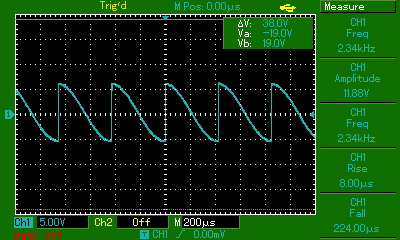
\includegraphics[width=0.5\textwidth]{bilder/MAP001.png}
    \caption{Phase 0° ohne Rauschen}        
    \label{fig:MAP001}
\end{figure}

\begin{figure}
    \centering
    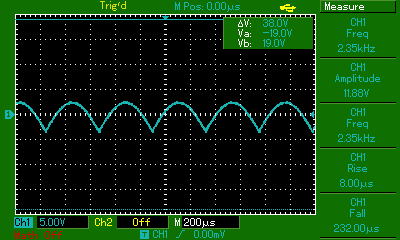
\includegraphics[width=0.5\textwidth]{bilder/MAP002.png}
    \caption{Phase 90° ohne Rauschen}        
    \label{fig:MAP002}
\end{figure}

\begin{figure}
    \centering
    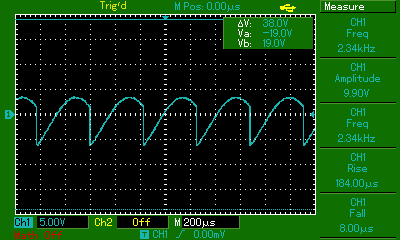
\includegraphics[width=0.5\textwidth]{bilder/MAP005.png}
    \caption{Phase 135° ohne Rauschen}        
    \label{fig:MAP005}
\end{figure}

\begin{figure}
    \centering
    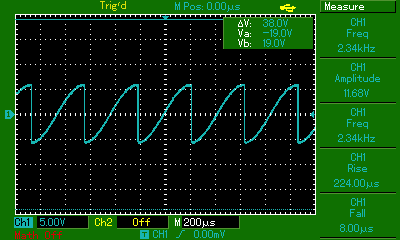
\includegraphics[width=0.5\textwidth]{bilder/MAP003.png}
    \caption{Phase 180° ohne Rauschen}        
    \label{fig:MAP003}
\end{figure}

\begin{figure}
    \centering
    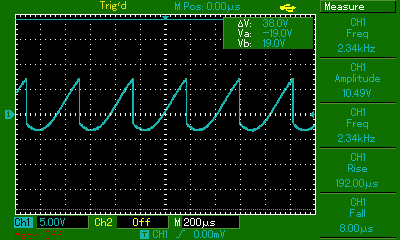
\includegraphics[width=0.5\textwidth]{bilder/MAP004.png}
    \caption{Phase 225° ohne Rauschen}        
    \label{fig:MAP004}
\end{figure}

\begin{figure}
    \centering
    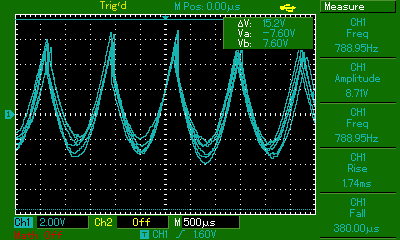
\includegraphics[width=0.5\textwidth]{bilder/MAP007.png}
    \caption{Phase 0° mit Rauschen}        
    \label{fig:MAP007}
\end{figure}

 \begin{figure}
     \centering
     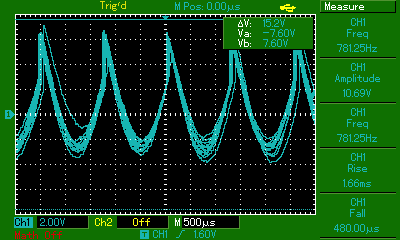
\includegraphics[width=0.5\textwidth]{bilder/MAP008.png}
     \caption{Phase 30° mit Rauschen}        
     \label{fig:MAP008}
 \end{figure}

\begin{figure}
    \centering
    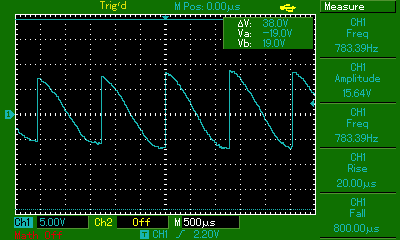
\includegraphics[width=0.5\textwidth]{bilder/MAP009.png}
    \caption{Phase 90° mit Rauschen}        
    \label{fig:MAP009}
\end{figure}

\begin{figure}
    \centering
    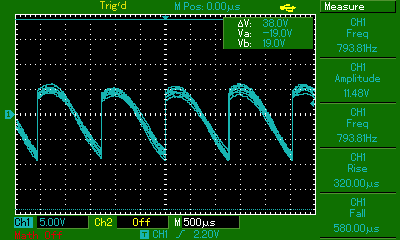
\includegraphics[width=0.5\textwidth]{bilder/MAP010.png}
    \caption{Phase 135° mit Rauschen}        
    \label{fig:MAP010}
\end{figure}

\begin{figure}
    \centering
    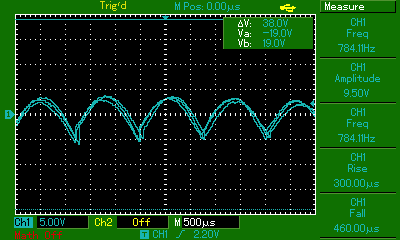
\includegraphics[width=0.5\textwidth]{bilder/MAP011.png}
    \caption{Phase 180° mit Rauschen}        
    \label{fig:MAP011}
\end{figure}

\begin{figure}
    \centering
    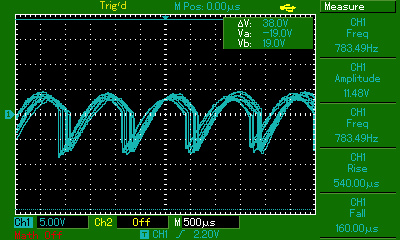
\includegraphics[width=0.5\textwidth]{bilder/MAP012.png}
    \caption{Phase 225° mit Rauschen}        
    \label{fig:MAP012}
\end{figure}

\begin{table}
    \centering
    \begin{tabular}{c c}
        \toprule
        $d\;/\;$cm & $U\;/\;$V\\
        \midrule
        0.0 & 0.0 \\ 
        30.0 & 1.5 \\ 
        60.0 & 3.5 \\ 
        90.0 & 4.0 \\ 
        120.0 & 3.75 \\ 
        150.0 & 2.0 \\ 
        180.0 & 0.5 \\ 
        210.0 & -1.0 \\ 
        240.0 & -3.0 \\ 
        270.0 & -3.5 \\ 
        300.0 & -3.0 \\ 
        330.0 & -1.5 \\ 
        360.0 & 0.0 \\ 
        \bottomrule
    \end{tabular}
    \caption{Messung der Spannung verschiedener Phasen}
    \label{tab:V1_Werte}
\end{table}
\begin{figure}
    \centering
    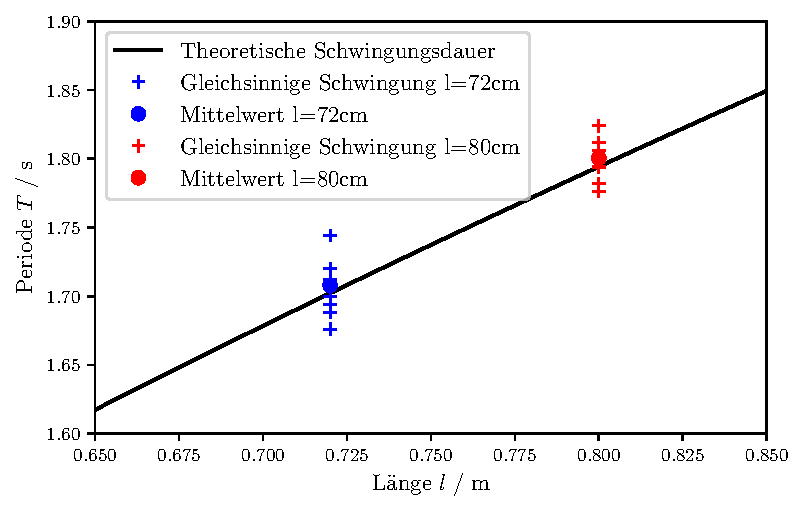
\includegraphics[width=0.5\textwidth]{build/plot1.pdf}
    \caption{Messwerte - Spannung in abhängigkeit von der Phase}        
    \label{fig:plot1}
\end{figure}

Die Spannung $U$ kann durch 
\begin{equation*}
    U_{out} = \frac{2}{\pi} A*cos(\frac{\phi}{180}\pi+B)
\end{equation*}
berechnet werden.
Durch eine Ausgleichsrechnung ergibt sich
\begin{align*}
    A=  -5.763 V\\
    B=  1.513
\end{align*}
\begin{table}
    \centering
    \begin{tabular}{c c}
        \toprule
        $d\;/\;$cm & $U\;/\;$V\\
        \midrule
        0.0 & -4.5 \\
        30.0 & -4.0 \\
        60.0 & -2.0 \\
        90.0 & -0.9 \\
        120.0 & 1.5 \\
        150.0 & 4.0 \\
        180.0 & 4.75 \\
        210.0 & 4.5 \\
        240.0 & 3.0 \\
        270.0 & 1.0 \\
        300.0 & -1.0 \\
        330.0 & -3.5 \\
        360.0 & -4.5 \\
        \bottomrule
    \end{tabular}
    \caption{Messung der Spannung verschiedener Phasen mit Rauschen}
    \label{tab:V2_Werte}
\end{table}

\begin{figure}
    \centering
    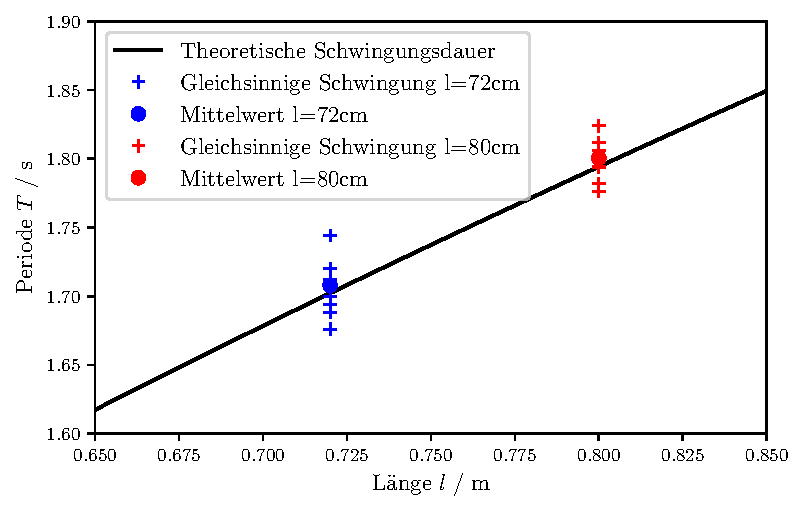
\includegraphics[width=0.5\textwidth]{build/plot1.pdf}
    \caption{Messwerte - Spannung in abhängigkeit von der Phase mit Rauschen}        
    \label{fig:plot2}
\end{figure}
Die Spannung $U$ kann wieder durch 
\begin{equation*}
    U_{out} = \frac{2}{\pi} A*cos(\frac{\phi}{180}\pi+B)
\end{equation*}
berechnet werden.
Durch eine weitere Ausgleichsrechnung ergibt sich
\begin{align*}
    A=  -7.137 V\\
    B=  6.115
\end{align*}
